\documentclass[11pt,letterpaper]{article}
\usepackage[top=0.85in,bottom=0.85in,left=1in,right=1in]{geometry}
\usepackage{amsmath,amssymb}
\usepackage{xcolor}
\usepackage{mdframed}
\usepackage{graphicx}
\usepackage{fancyhdr}
\usepackage{booktabs}
\usepackage{colortbl}
\usepackage{cancel}

\graphicspath{{cs_crops/}{./}}

\definecolor{teal}{HTML}{0F6E56}\definecolor{tealbg}{HTML}{E1F5EE}
\definecolor{coral}{HTML}{993C1D}\definecolor{coralbg}{HTML}{FAECE7}
\definecolor{purple}{HTML}{534AB7}\definecolor{purplebg}{HTML}{EEEDFE}
\definecolor{amber}{HTML}{854F0B}\definecolor{amberbg}{HTML}{FAEEDA}

\newmdenv[linewidth=1pt,linecolor=teal,backgroundcolor=tealbg!30,
  innerleftmargin=6pt,innerrightmargin=6pt,
  innertopmargin=4pt,innerbottommargin=4pt,
  skipabove=4pt,skipbelow=6pt]{cssnip}

\newmdenv[linewidth=1pt,linecolor=coral,backgroundcolor=coralbg!30,
  innerleftmargin=6pt,innerrightmargin=6pt,
  innertopmargin=4pt,innerbottommargin=4pt,
  skipabove=4pt,skipbelow=4pt]{notebox}

\newmdenv[linewidth=0.8pt,linecolor=purple,backgroundcolor=purplebg!20,
  innerleftmargin=6pt,innerrightmargin=6pt,
  innertopmargin=3pt,innerbottommargin=3pt,
  skipabove=4pt,skipbelow=4pt]{goalbox}

\pagestyle{fancy}\fancyhf{}
\renewcommand{\headrulewidth}{0.4pt}
\fancyhead[L]{\textbf{ECE332 Spring 2026 --- HW4 Generated Answers}}
\fancyhead[R]{Bao Nguyen}
\fancyfoot[C]{\thepage}

\setlength{\parindent}{0pt}\setlength{\parskip}{4pt}

\newcommand{\probhead}[2]{%
  \colorbox{purplebg}{\parbox{\dimexpr\linewidth-2\fboxsep}%
  {\color{purple}\large\textbf{Problem #1 \hfill #2}}}}

\newcommand{\goal}[1]{\textbf{\color{purple}Goal:} #1}
\newcommand{\need}[1]{\textbf{\color{coral}Need:} #1}

\begin{document}

\begin{center}
{\Large\textbf{ECE 332 --- Homework 4: Generated Answers from HW4 Cheat Sheet}}\\[4pt]
{\small Each problem: state the goal equation $\to$ identify missing variables $\to$ solve each $\to$ plug back $\to$ box the answer.}
\end{center}

\vspace{4pt}

\begin{notebox}
\textbf{Symbol reference} (used throughout):
\begin{itemize}\setlength{\itemsep}{0pt}\setlength{\topsep}{1pt}\setlength{\parsep}{0pt}
\item $l$ --- antenna physical length (m)
\item $\lambda = c/f$ --- wavelength (m); $c=3\!\times\!10^8$ m/s
\item $I_0$ --- peak current at antenna feed (A)
\item $R$ --- distance from antenna to observation point (m)
\item $\theta$ --- angle from antenna axis (rad or deg)
\item $\eta_0 = 120\pi \approx 377\,\Omega$ --- intrinsic impedance of free space
\item $k = 2\pi/\lambda$ --- wavenumber (rad/m)
\item $S(R,\theta)$ --- average power density radiated (W/m\textsuperscript{2})
\item $F(\theta) = S(\theta)/S_{\max}$ --- normalized radiation intensity (unitless)
\item $\beta$ --- half-power beamwidth (rad or deg)
\item $\Omega_p$ --- pattern solid angle (sr)
\item $D = 4\pi/\Omega_p$ --- directivity (unitless, often dB)
\item $A_e = \lambda^2 D/(4\pi)$ --- effective aperture area (m\textsuperscript{2})
\item $A_p$ --- physical cross-section area (m\textsuperscript{2})
\item $G_t, G_r$ --- antenna gains (linear)
\item $P_t, P_r$ --- transmitted / received power (W)
\item $k_B = 1.38\!\times\!10^{-23}$ J/K --- Boltzmann constant
\item $T_{\text{sys}}$ --- system noise temperature (K)
\item $B$ --- receiver bandwidth (Hz)
\end{itemize}
\textit{\color{coral}\textbf{Key shortcuts:} Hertzian dipole ($l/\lambda < 1/50$) $\Rightarrow D = 1.5$. Half-wave dipole ($l = \lambda/2$) $\Rightarrow D = 1.64$, $R_{\text{rad}} = 73.2\,\Omega$. 3 dB $\Rightarrow$ linear gain of 2.}
\end{notebox}

\vspace{4pt}

%======================================================
\probhead{1 --- Hertzian Dipole Power Density at 5 km}{8 pts}

\textbf{Setup:} $l = 1$ m, $f = 1$ MHz, $I_0 = 12$ A, $R = 5$ km, $\theta = 45^\circ$. Find $S(R,\theta)$.

\begin{cssnip}
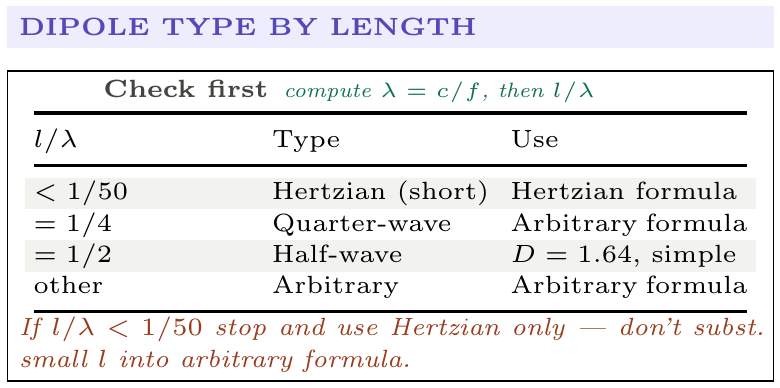
\includegraphics[width=0.49\linewidth]{cs_dipole_type}\hfill
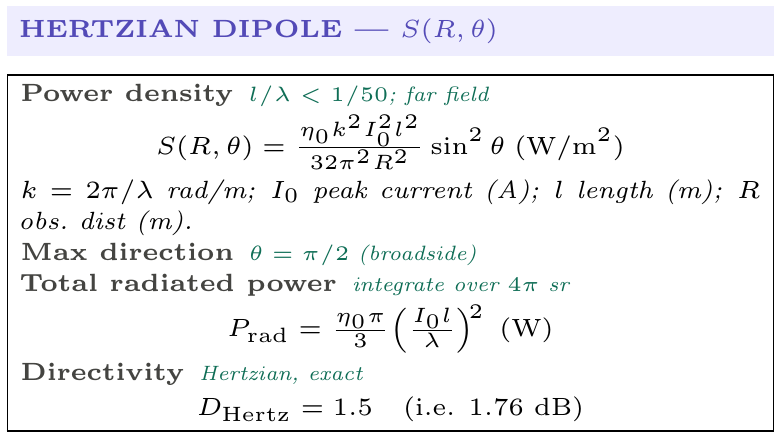
\includegraphics[width=0.49\linewidth]{cs_hertzian}\\[3pt]
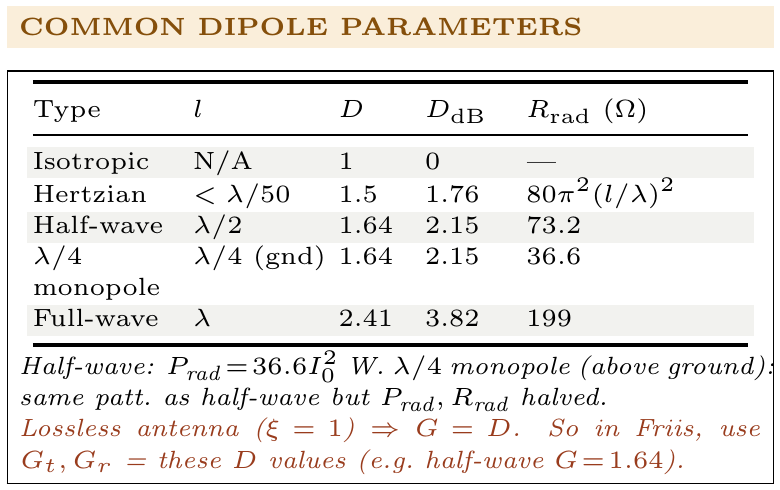
\includegraphics[width=0.49\linewidth]{cs_dipole_params}
\end{cssnip}

\textbf{Step 0 --- Classify the dipole.} From DIPOLE TYPE BY LENGTH, we need $l/\lambda$.
\[\lambda = \tfrac{c}{f} = \tfrac{3\!\times\!10^8}{10^6} = 300~\text{m},\quad \tfrac{l}{\lambda} = \tfrac{1}{300} < \tfrac{1}{50}\;\Rightarrow\;\textbf{Hertzian}\]

\begin{goalbox}
\goal{find $S(R,\theta)$ using the Hertzian power density formula (from HERTZIAN DIPOLE box):}
\[S(R,\theta) = \tfrac{\eta_0 k^2 I_0^2 l^2}{32\pi^2 R^2}\sin^2\theta\]
\need{$\eta_0$, $k$, $I_0$, $l$, $R$, $\theta$.}
\end{goalbox}

\textbf{Solve each unknown:}

\textit{$\eta_0$:} constant, free-space impedance.
\[\eta_0 = 120\pi\,\Omega\]

\textit{$k$:} wavenumber from wavelength.
\[k = \tfrac{2\pi}{\lambda} = \tfrac{2\pi}{300}\;\text{rad/m}\]

\textit{$I_0, l, R, \theta$:} given.
\[I_0 = 12~\text{A},\quad l = 1~\text{m},\quad R = 5000~\text{m},\quad \theta = 45^\circ\]

\textbf{Plug back in:}
\[S = \tfrac{(120\pi)(2\pi/300)^2(12)^2(1)^2}{32\pi^2(5000)^2}\sin^2(45^\circ)\]
With $\sin^2(45^\circ) = 1/2$:
\[S = \tfrac{(120\pi)(4\pi^2/90000)(144)(1)}{32\pi^2(25{\times}10^6)} \cdot \tfrac{1}{2}\]
Simplify: numerator has $120\pi \cdot 4\pi^2 \cdot 144 / 90000 = 69120\pi^3/90000$, denominator $32\pi^2 \cdot 25\!\times\!10^6 = 8\!\times\!10^8 \pi^2$. Combine and multiply by $1/2$:
\[\boxed{S(5\text{ km},\,45^\circ) = 1.51\!\times\!10^{-9}~\text{W/m}^2 = 1.51~\text{nW/m}^2}\]

\textit{Sanity:} 12 A at 1 MHz through 1 m radiates 1.5 nW/m\textsuperscript{2} at 5 km. The $1/R^2$ falloff dominates — most power scatters into space, only a tiny fraction reaches any one point.

\newpage
%======================================================
\probhead{2 --- Beam Parameters from $F(\theta) = e^{-20\theta^2}$}{15 pts}

\textbf{Setup:} $F(\theta) = \exp(-20\theta^2)$ for $0 \le \theta \le \pi$ ($\theta$ in radians). Find (a) HPBW $\beta$, (b) $\Omega_p$, (c) $D$.

\begin{cssnip}
\begin{center}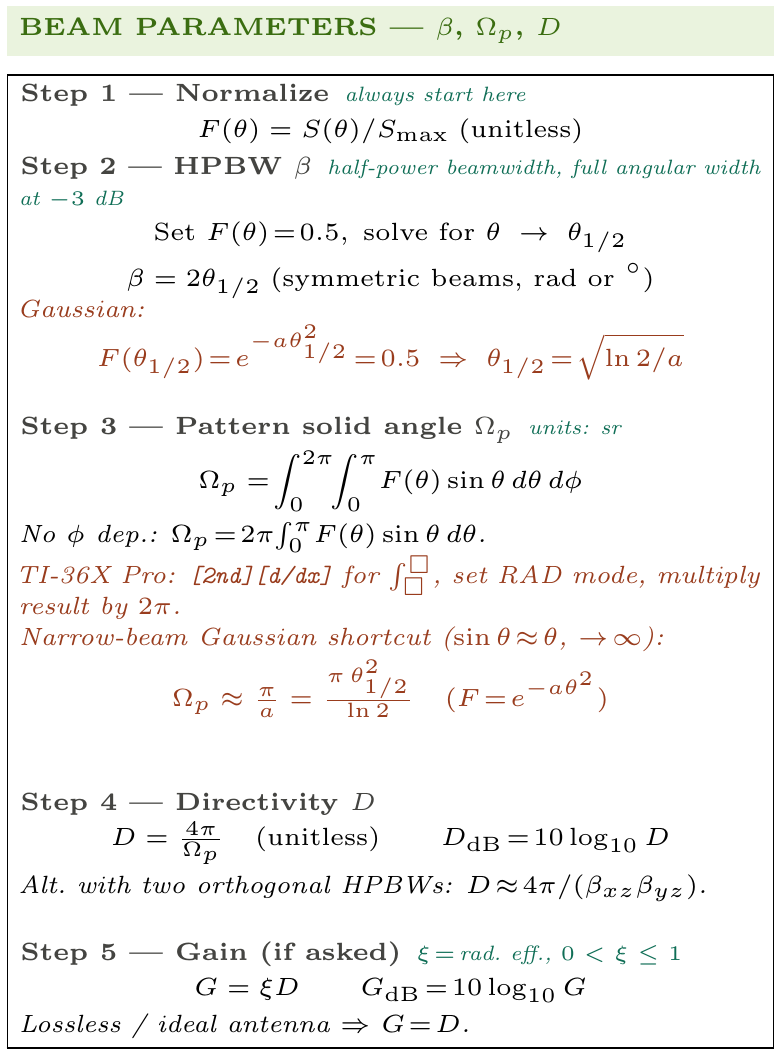
\includegraphics[width=0.55\linewidth]{cs_beam}\end{center}
\end{cssnip}

\textbf{(a) Half-power beamwidth $\beta$ (5 pts)}

\begin{goalbox}
\goal{find $\beta$ using the HPBW procedure (BEAM PARAMETERS Step 2):}
\[\text{Set }F(\theta) = 0.5,\;\text{solve for }\theta \to \theta_{1/2}\]
\[\beta = 2\theta_{1/2}\quad(\text{symmetric beam})\]
\need{$\theta_{1/2}$, found by setting our specific $F(\theta) = 0.5$.}
\end{goalbox}

\textbf{Solve $\theta_{1/2}$:} plug $F = \exp(-20\theta^2)$:
\[\exp(-20\theta_{1/2}^2) = 0.5\;\Rightarrow\;-20\theta_{1/2}^2 = \ln(0.5) = -0.693\]
\[\theta_{1/2}^2 = \tfrac{0.693}{20} = 0.03466,\quad \theta_{1/2} = \sqrt{0.03466} = 0.186~\text{rad}\]

That's the half-angle from peak to one $-3$ dB point. Since the beam is symmetric about $\theta = 0$, the \emph{full} half-power beamwidth is twice that:
\[\boxed{\beta = 2\theta_{1/2} = 0.372~\text{rad} = 21.31^\circ}\]

\vspace{6pt}
\textbf{(b) Pattern solid angle $\Omega_p$ (5 pts)}

\begin{goalbox}
\goal{find $\Omega_p$ using the integral definition (BEAM PARAMETERS Step 3):}
\[\Omega_p = \iint_{4\pi} F(\theta)\sin\theta\,d\theta\,d\phi\]
\need{evaluate this integral with our specific $F(\theta) = e^{-20\theta^2}$.}
\end{goalbox}

\textbf{Set up the integral:} $F$ has no $\phi$ dependence, so $\int_0^{2\pi} d\phi = 2\pi$:
\[\Omega_p = 2\pi\!\int_0^{\pi} e^{-20\theta^2}\sin\theta\,d\theta\]

\textbf{Solve numerically on TI-36X Pro} (no closed form):
\begin{enumerate}\setlength{\itemsep}{0pt}
  \item \texttt{[mode]} $\to$ \textbf{RAD}
  \item \texttt{[2nd][d/dx]} for $\int_\square^\square$ template
  \item Lower limit: \texttt{0}; Upper limit: \texttt{[$\pi$]}
  \item Integrand: \texttt{e\^{}(-20$\times$x\^{}2)$\times$sin(x)}
  \item Variable: \texttt{x}; \texttt{[enter]} $\to$ returns $\approx 0.024792$
  \item Multiply: \texttt{$\times$[$\pi$]$\times$2 [enter]} $\to$ $\approx 0.15578$
\end{enumerate}

\[\boxed{\Omega_p \approx 0.1558~\text{sr}}\]
\textit{Keep the unrounded value for part (c). Textbook rounds to $0.156$ first and gets $D = 80.55$; using full precision gives $D \approx 80.67$.}

\vspace{6pt}
\textbf{(c) Directivity $D$ (5 pts)}

\begin{goalbox}
\goal{find $D$ using the standard formula (BEAM PARAMETERS Step 4):}
\[D = \tfrac{4\pi}{\Omega_p}\]
\need{$\Omega_p$ (from part b).}
\end{goalbox}

\textbf{Plug in:} $\Omega_p = 0.15578$ sr:
\[D = \tfrac{4\pi}{0.15578} = \tfrac{12.566}{0.15578}\]
\[\boxed{D = 80.67}\]
\textit{In dB: $D_{\text{dB}} = 10\log_{10}(80.67) = 19.07$ dB.}

\textit{Sanity:} $D \approx 80$ is highly directive (much narrower than half-wave's $D = 1.64$). The narrow Gaussian-like beam ($\beta \approx 21^\circ$) concentrates radiation into a small solid angle, so directivity is large.

\newpage
%======================================================
\probhead{3 --- $\lambda/4$ Dipole Radiation Pattern}{15 pts}

\textbf{Setup:} Dipole of length $l = \lambda/4$. Find (a) $\theta_{\max}$, (b) $S_{\max}$, (c) plot $F(\theta)$.

\begin{cssnip}
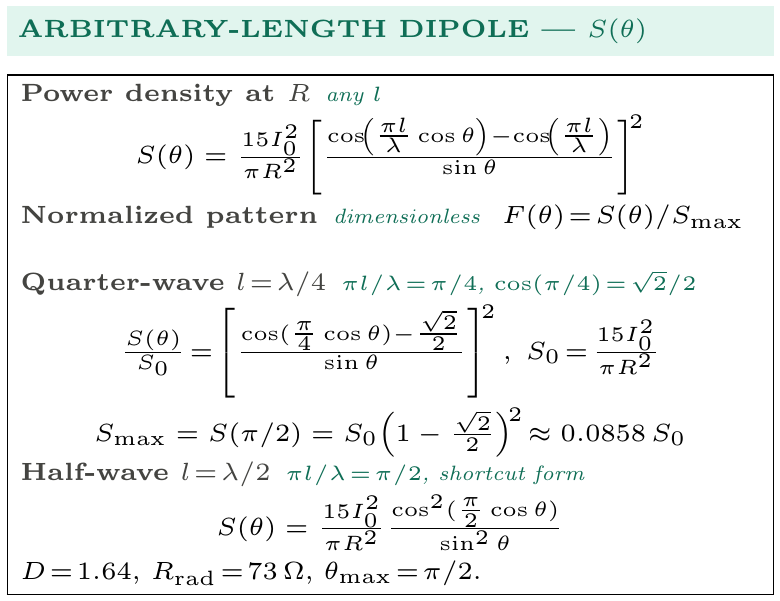
\includegraphics[width=0.49\linewidth]{cs_arbdipole}\hfill
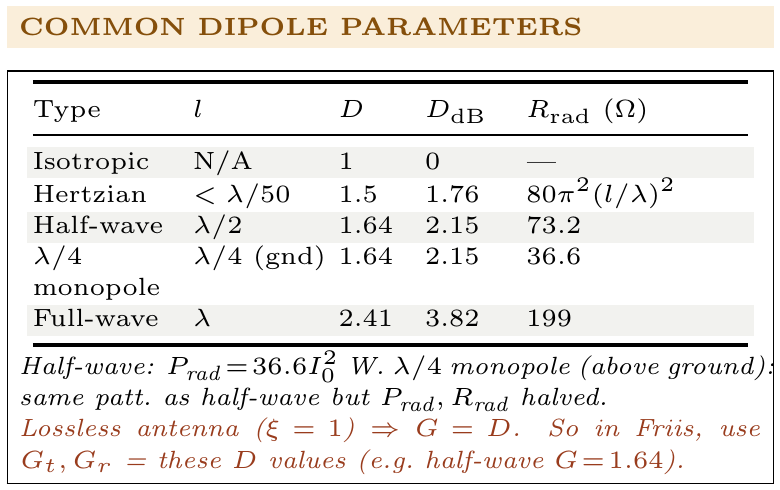
\includegraphics[width=0.49\linewidth]{cs_dipole_params}\\[3pt]
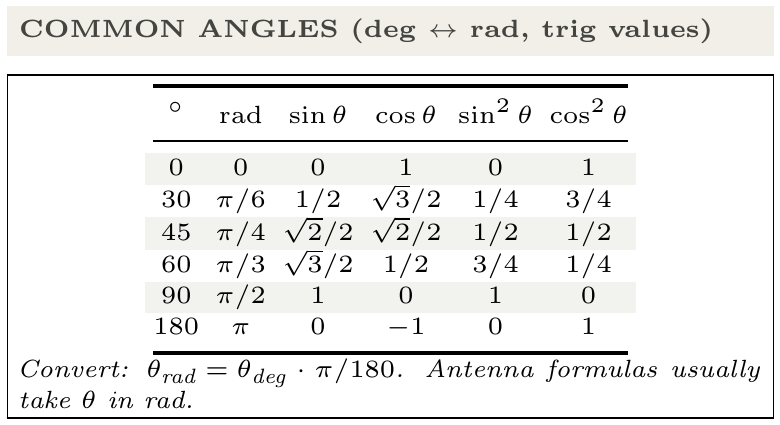
\includegraphics[width=0.65\linewidth]{cs_angles}
\end{cssnip}

\textbf{Common setup for all 3 parts.}

\begin{goalbox}
\goal{starting point for parts (a)-(c) is the arbitrary-length dipole power density (from ARBITRARY-LENGTH DIPOLE box):}
\[S(\theta) = \tfrac{15 I_0^2}{\pi R^2}\!\left[\tfrac{\cos\!\left(\tfrac{\pi l}{\lambda}\cos\theta\right) - \cos\!\left(\tfrac{\pi l}{\lambda}\right)}{\sin\theta}\right]^2\]
\need{plug in $l = \lambda/4$ to simplify.}
\end{goalbox}

\textbf{Substitute $l = \lambda/4 \Rightarrow \pi l/\lambda = \pi/4$:}
\[S(\theta) = \tfrac{15 I_0^2}{\pi R^2}\!\left[\tfrac{\cos\!\left(\tfrac{\pi}{4}\cos\theta\right) - \cos(\pi/4)}{\sin\theta}\right]^2\]
From COMMON ANGLES table: $\cos(\pi/4) = \sqrt{2}/2 = 0.7071$.
\[S(\theta) = S_0\!\left[\tfrac{\cos\!\left(\tfrac{\pi}{4}\cos\theta\right) - \tfrac{\sqrt{2}}{2}}{\sin\theta}\right]^2,\quad S_0 \equiv \tfrac{15 I_0^2}{\pi R^2}\]

\vspace{6pt}
\textbf{(a) Direction of maximum radiation $\theta_{\max}$ (5 pts)}

\begin{goalbox}
\goal{find $\theta_{\max}$ where $S(\theta)$ is maximum.}
\need{know the shape of $S(\theta)$ over $\theta \in [0, \pi]$. Three-step argument: endpoints, symmetry, sampling.}
\end{goalbox}

\textit{Step (i) --- endpoints via L'H\^opital.} Define $f(\theta) = \cos\!\left(\tfrac{\pi}{4}\cos\theta\right) - \tfrac{\sqrt{2}}{2}$ and $g(\theta) = \sin\theta$. At $\theta = 0$:
\[f(0) = \cos(\pi/4 \cdot 1) - \sqrt{2}/2 = \sqrt{2}/2 - \sqrt{2}/2 = 0\]
\[g(0) = \sin(0) = 0 \Rightarrow \text{0/0 form, apply L'H\^opital.}\]
Derivatives (chain rule for $f$):
\[f'(\theta) = \tfrac{\pi}{4}\sin\!\left(\tfrac{\pi}{4}\cos\theta\right)\sin\theta,\quad g'(\theta) = \cos\theta\]
\[\lim_{\theta\to 0}\tfrac{f'(\theta)}{g'(\theta)} = \tfrac{(\pi/4)\sin(\pi/4)\cdot 0}{1} = 0\]
So $S(0)/S_0 = 0^2 = 0$. Same algebra at $\theta = \pi$: $S(\pi) = 0$. \textbf{Peak is in $(0, \pi)$.}

\textit{Step (ii) --- symmetry.} Substitute $\theta \to \pi - \theta$: $\cos(\pi-\theta) = -\cos\theta$, but $\cos$ is even so $\cos((\pi/4)\cos(\pi-\theta)) = \cos((\pi/4)\cos\theta)$. And $\sin(\pi-\theta) = \sin\theta$. So $S(\theta) = S(\pi-\theta)$. \textbf{Pattern mirrors about $\theta = \pi/2$.}

\textit{Step (iii) --- sample to confirm single peak.}

At $\theta = 30^\circ$: $\cos(30^\circ) = 0.866$, $(\pi/4)(0.866) = 0.680$, $\cos(0.680) = 0.777$, $0.777-0.707 = 0.070$, $\sin(30^\circ) = 0.500$, $0.070/0.500 = 0.140$, $(0.140)^2 = \mathbf{0.020}$.

At $\theta = 60^\circ$: $\cos(60^\circ) = 0.500$, $(\pi/4)(0.500) = 0.393$, $\cos(0.393) = 0.924$, $0.924-0.707 = 0.217$, $\sin(60^\circ) = 0.866$, $0.217/0.866 = 0.250$, $(0.250)^2 = \mathbf{0.063}$.

At $\theta = 90^\circ$: $\cos(90^\circ) = 0$, $(\pi/4)(0) = 0$, $\cos(0) = 1$, $1-0.707 = 0.293$, $\sin(90^\circ) = 1$, $0.293/1 = 0.293$, $(0.293)^2 = \mathbf{0.0858}$.

\begin{center}
\begin{tabular}{cccc}
\toprule
$\theta$ & $30^\circ$ & $60^\circ$ & $90^\circ$\\
\midrule
$S/S_0$ & 0.020 & 0.063 & \textbf{0.0858}\\
\bottomrule
\end{tabular}
\end{center}
Monotone rise to $90^\circ$, then symmetric fall (by step (ii)). Single peak at the center.
\[\boxed{\theta_{\max} = \pi/2 = 90^\circ\;\text{(broadside)}}\]

\vspace{6pt}
\textbf{(b) Expression for $S_{\max}$ (5 pts)}

\begin{goalbox}
\goal{find $S_{\max}$ by evaluating $S$ at the maximum direction:}
\[S_{\max} = S(\theta_{\max})\]
\need{$\theta_{\max}$ (from part a: $\theta_{\max} = \pi/2$).}
\end{goalbox}

\textbf{Plug $\theta = \pi/2$ into $S(\theta)$ step by step:}

\textit{Inner cos:}\ $\cos(\pi/2) = 0$, so $\tfrac{\pi}{4}\cos(\pi/2) = 0$.

\textit{Outer cos:}\ $\cos(0) = 1$.

\textit{Denominator:}\ $\sin(\pi/2) = 1$.

\textit{Bracket:}\ $(1 - \sqrt{2}/2)/1 = 1 - \sqrt{2}/2 = 1 - 0.7071 = 0.2929$.

\textit{Square:}\ $(0.2929)^2 = 0.0858$.

\textit{Multiply by $S_0$:}
\[\boxed{S_{\max} = 0.0858\cdot\tfrac{15 I_0^2}{\pi R^2} \approx \tfrac{1.287\,I_0^2}{\pi R^2}}\]

\vspace{6pt}
\textbf{(c) Normalized pattern $F(\theta) = S(\theta)/S_{\max}$ (5 pts)}

\begin{goalbox}
\goal{find $F(\theta)$ by dividing $S(\theta)$ by $S_{\max}$, then plot.}
\need{$S(\theta)$ and $S_{\max}$ (both from above).}
\end{goalbox}

\textbf{Compute the normalization coefficient:}\ $1/0.0858 = 11.66$.

\textbf{Form $F(\theta)$:}
\[\boxed{F(\theta) = 11.66\!\left[\tfrac{\cos\!\left(\tfrac{\pi}{4}\cos\theta\right) - \tfrac{\sqrt{2}}{2}}{\sin\theta}\right]^2}\]

\textbf{Plot:} bell-shaped curve peaking at $\theta = \pi/2$ with $F = 1$, dropping to 0 at $\theta = 0$ and $\pi$. Symmetric about $\theta = \pi/2$. Similar shape to half-wave dipole pattern but slightly narrower since the dipole is shorter.

\newpage
%======================================================
\probhead{4 --- Effective Area vs.\ Physical Cross-section}{5 pts}

\textbf{Setup:} Half-wave dipole at $f = 100$ MHz, wire diameter $d = 2$ cm. Find $A_e$ and compare to $A_p$.

\begin{cssnip}
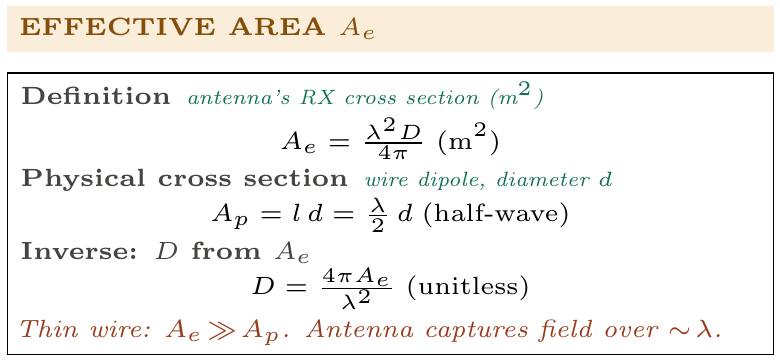
\includegraphics[width=0.49\linewidth]{cs_aeff}\hfill
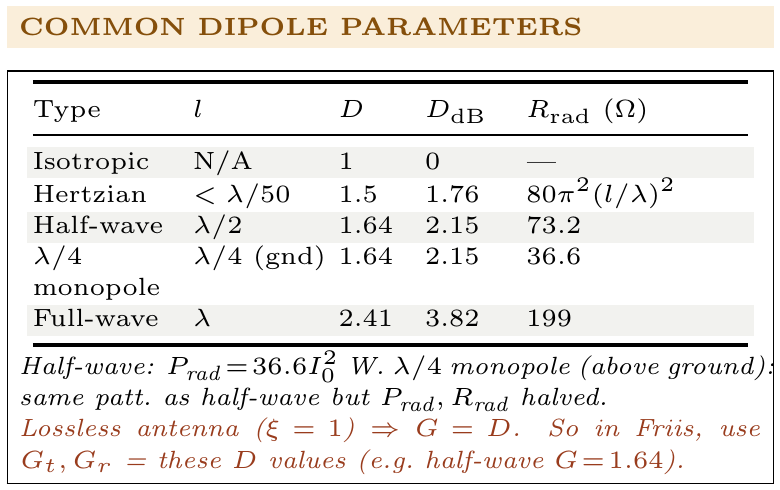
\includegraphics[width=0.49\linewidth]{cs_dipole_params}
\end{cssnip}

\textbf{Part 1 --- Effective area $A_e$}

\begin{goalbox}
\goal{find $A_e$ using the standard formula (from EFFECTIVE AREA box):}
\[A_e = \tfrac{\lambda^2 D}{4\pi}\]
\need{$\lambda$ and $D$.}
\end{goalbox}

\textbf{Solve each unknown:}

\textit{$\lambda$:} use $\lambda = c/f$.
\[\lambda = \tfrac{c}{f} = \tfrac{3\!\times\!10^8}{10^8} = 3~\text{m}\]

\textit{$D$:} look up half-wave in COMMON DIPOLE PARAMETERS table.
\[D_{\text{half-wave}} = 1.64\]

\textbf{Plug back in:}
\[A_e = \tfrac{(3)^2(1.64)}{4\pi} = \tfrac{9\cdot 1.64}{4\pi} = \tfrac{14.76}{12.566}\]
\[\boxed{A_e = 1.17~\text{m}^2}\]

\vspace{6pt}
\textbf{Part 2 --- Physical cross-section $A_p$}

\begin{goalbox}
\goal{find $A_p$ using the wire-dipole formula:}
\[A_p = l \cdot d\]
\need{$l$ and $d$.}
\end{goalbox}

\textbf{Solve each unknown:}

\textit{$l$:} half-wave means $l = \lambda/2$ (from COMMON DIPOLE PARAMS table).
\[l = \tfrac{\lambda}{2} = \tfrac{3}{2} = 1.5~\text{m}\]

\textit{$d$:} given.
\[d = 2~\text{cm} = 0.02~\text{m}\]

\textbf{Plug back in:}
\[A_p = (1.5)(0.02) = \boxed{0.03~\text{m}^2}\]

\vspace{6pt}
\textbf{Part 3 --- Ratio}
\[\tfrac{A_e}{A_p} = \tfrac{1.17}{0.03} = \boxed{39.2}\]

\textit{Sanity:} the antenna's "catching area" is 39$\times$ its physical wire cross-section. A thin wire interacts with the field over a region $\sim \lambda$ around itself, so it captures much more energy than its tiny wire would suggest.

\newpage
%======================================================
\probhead{5 --- Friis Transmission, TV Broadcast}{5 pts}

\textbf{Setup:} Half-wave dipole TX, $P_t = 1$ kW at $f = 50$ MHz. RX antenna with $G_r = 3$ dB, distance $R = 30$ km. Find $P_r$.

\begin{cssnip}
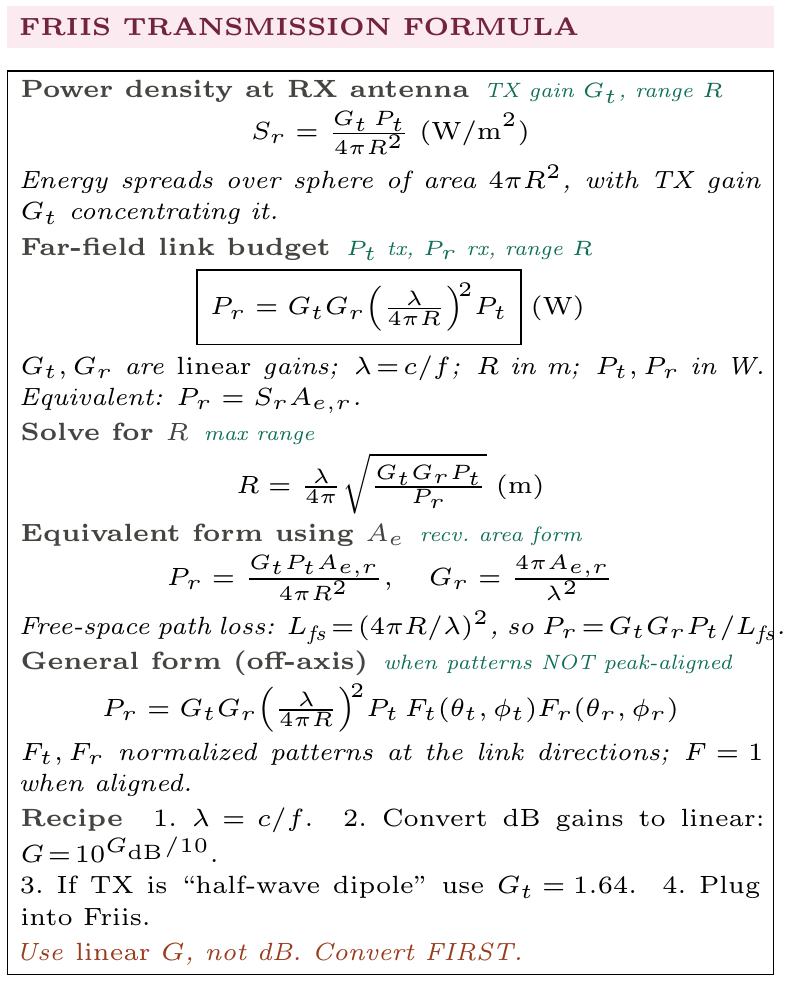
\includegraphics[width=0.49\linewidth]{cs_friis}\hfill
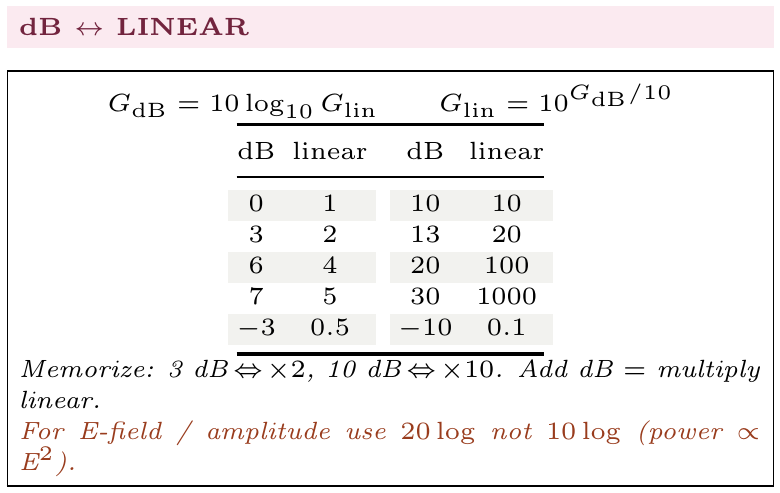
\includegraphics[width=0.49\linewidth]{cs_db}
\end{cssnip}

\begin{goalbox}
\goal{find $P_r$ using the Friis transmission formula (from FRIIS TRANSMISSION FORMULA box):}
\[P_r = G_t G_r\!\left(\tfrac{\lambda}{4\pi R}\right)^{\!2}\!P_t\]
\need{$G_t$, $G_r$ (both linear), $\lambda$, $R$, $P_t$.}
\end{goalbox}

\textbf{Solve each unknown:}

\textit{$\lambda$:} $\lambda = c/f$.
\[\lambda = \tfrac{3\!\times\!10^8}{5\!\times\!10^7} = 6~\text{m}\]

\textit{$G_t$:} TX is half-wave dipole, COMMON DIPOLE PARAMS gives $D = 1.64$, and for lossless antenna $G = D$.
\[G_t = 1.64\]

\textit{$G_r$:} given as 3 dB. Convert to linear via dB $\to$ LINEAR table: 3 dB $= \times 2$.
\[G_r = 10^{3/10} = 2\]

\textit{$R$, $P_t$:} given.
\[R = 30~\text{km} = 3\!\times\!10^4~\text{m},\quad P_t = 10^3~\text{W}\]

\textbf{Plug back in:} compute the path-loss factor first.
\[\tfrac{\lambda}{4\pi R} = \tfrac{6}{4\pi(3\!\times\!10^4)} = \tfrac{6}{3.77\!\times\!10^5} = 1.59\!\times\!10^{-5}\]
\[\left(\tfrac{\lambda}{4\pi R}\right)^{\!2} = (1.59\!\times\!10^{-5})^2 = 2.53\!\times\!10^{-10}\]
\[P_r = (1.64)(2)(2.53\!\times\!10^{-10})(10^3) = (3.28)(2.53\!\times\!10^{-7})\]
\[\boxed{P_r = 8.3\!\times\!10^{-7}~\text{W} = 0.83~\mu\text{W}}\]

\textit{Sanity:} 1 kW in, 0.83 $\mu$W out at 30 km. A 90 dB drop, dominated by $1/R^2$ path loss. Plenty for a TV receiver (sensitivity $\sim 10^{-13}$ W).

\newpage
%======================================================
\probhead{6 --- Communication Link with SNR}{15 pts (new)}

\textbf{Setup:} $G_t = 20$ dB, $G_r = 23$ dB, $R = 20$ km, $P_t = 10$ W, $f = 6$ GHz. (c) $T_{\text{sys}} = 1000$ K, $B = 20$ MHz.

\begin{cssnip}
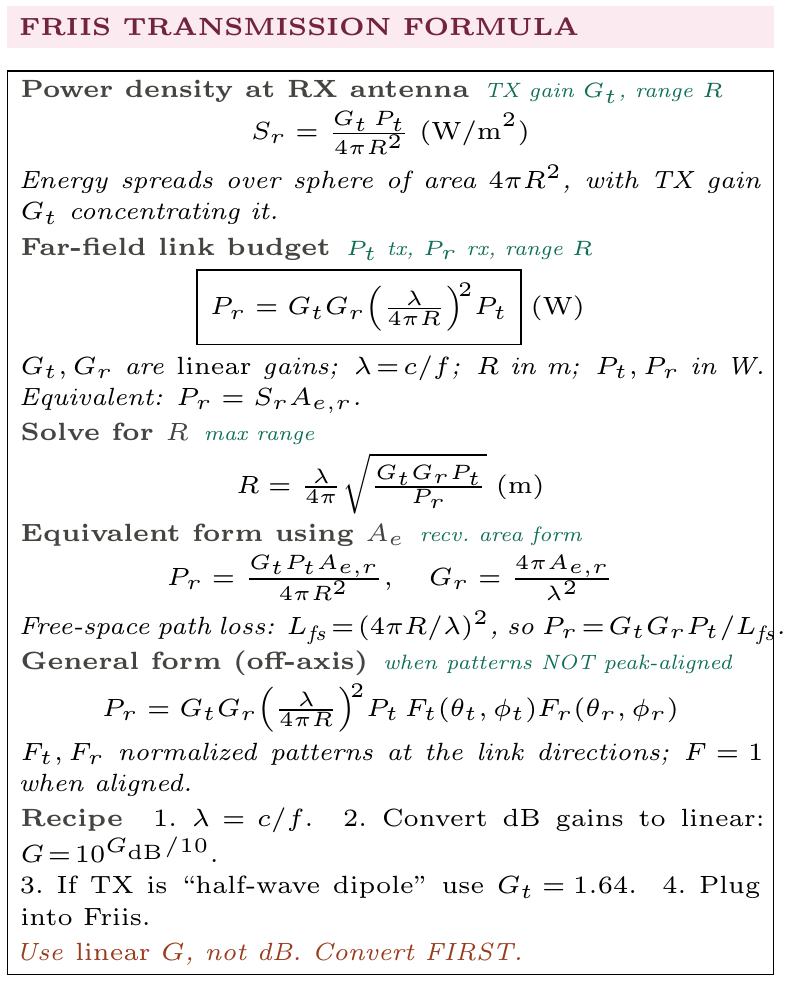
\includegraphics[width=0.49\linewidth]{cs_friis}\hfill
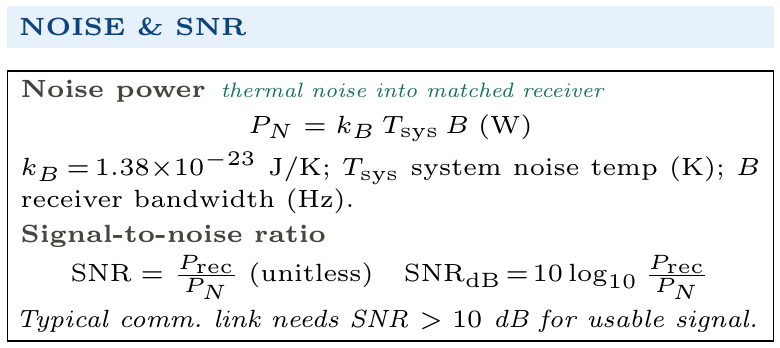
\includegraphics[width=0.49\linewidth]{cs_noise}\\[3pt]
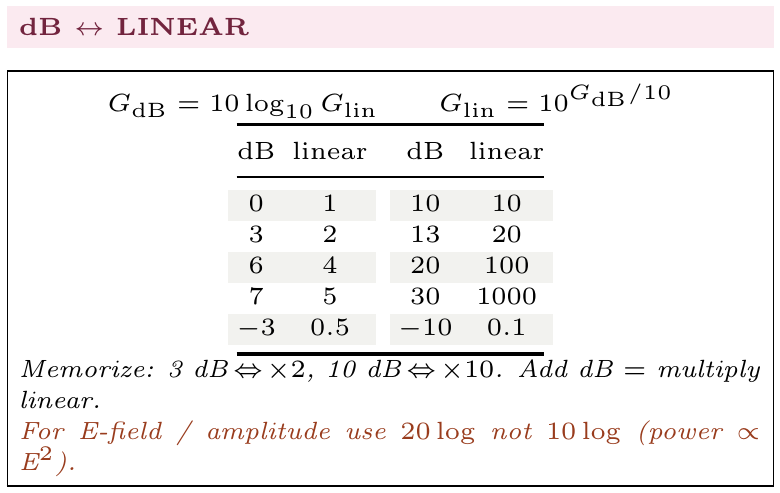
\includegraphics[width=0.49\linewidth]{cs_db}
\end{cssnip}

\textbf{Shared setup:} convert dB to linear and compute $\lambda$.
\[\lambda = \tfrac{c}{f} = \tfrac{3\!\times\!10^8}{6\!\times\!10^9} = 0.05~\text{m}\]
\[G_t = 10^{20/10} = 100,\quad G_r = 10^{23/10} = 199.5\]

\vspace{6pt}
\textbf{(a) Power density at RX antenna $S_r$ (5 pts)}

\begin{goalbox}
\goal{find $S_r$ using power-spreading-over-sphere (with TX gain factored in):}
\[S_r = \tfrac{G_t\,P_t}{4\pi R^2}\]
\need{$G_t$, $P_t$, $R$.}
\end{goalbox}

\textbf{Plug in:}
\[S_r = \tfrac{(100)(10)}{4\pi(2\!\times\!10^4)^2} = \tfrac{1000}{4\pi(4\!\times\!10^8)} = \tfrac{1000}{5.027\!\times\!10^9}\]
\[\boxed{S_r = 1.989\!\times\!10^{-7}~\text{W/m}^2 \approx 0.199~\mu\text{W/m}^2}\]

\vspace{6pt}
\textbf{(b) Received power $P_r$ (5 pts)}

\begin{goalbox}
\goal{find $P_r$ using Friis (from FRIIS TRANSMISSION box):}
\[P_r = G_t G_r\!\left(\tfrac{\lambda}{4\pi R}\right)^{\!2}\!P_t\]
\need{$G_t$, $G_r$, $\lambda$, $R$, $P_t$ (all already converted).}
\end{goalbox}

\textbf{Plug in:}
\[\tfrac{\lambda}{4\pi R} = \tfrac{0.05}{4\pi(2\!\times\!10^4)} = 1.989\!\times\!10^{-7}\]
\[\left(\tfrac{\lambda}{4\pi R}\right)^{\!2} = 3.957\!\times\!10^{-14}\]
\[P_r = (100)(199.5)(3.957\!\times\!10^{-14})(10) = 7.894\!\times\!10^{-9}\]
\[\boxed{P_r = 7.89~\text{nW}}\]

\textit{Cross-check via effective area:} $A_{e,r} = G_r\lambda^2/(4\pi) = 199.5(0.0025)/(4\pi) = 0.0397$ m\textsuperscript{2}, then $P_r = S_r A_{e,r} = (1.989\!\times\!10^{-7})(0.0397) = 7.89\!\times\!10^{-9}$ W $\checkmark$.

\vspace{6pt}
\textbf{(c) Signal-to-noise ratio in dB (5 pts)}

\begin{goalbox}
\goal{find SNR in dB. From NOISE \& SNR box, two steps:}
\[P_N = k_B\,T_{\text{sys}}\,B\quad\text{then}\quad\text{SNR}_{\text{dB}} = 10\log_{10}\tfrac{P_r}{P_N}\]
\need{$P_N$ first ($\to$ need $k_B$, $T_{\text{sys}}$, $B$), then $P_r$ (from part b).}
\end{goalbox}

\textbf{Solve each unknown:}

\textit{$k_B$:} Boltzmann constant.
\[k_B = 1.38\!\times\!10^{-23}~\text{J/K}\]

\textit{$T_{\text{sys}}$, $B$:} given.
\[T_{\text{sys}} = 1000~\text{K},\quad B = 20~\text{MHz} = 2\!\times\!10^7~\text{Hz}\]

\textbf{Compute $P_N$:}
\[P_N = (1.38\!\times\!10^{-23})(1000)(2\!\times\!10^7) = 2.76\!\times\!10^{-13}~\text{W}\]

\textbf{Compute SNR:}
\[\text{SNR}_{\text{lin}} = \tfrac{P_r}{P_N} = \tfrac{7.89\!\times\!10^{-9}}{2.76\!\times\!10^{-13}} = 2.86\!\times\!10^4\]
\[\boxed{\text{SNR}_{\text{dB}} = 10\log_{10}(2.86\!\times\!10^4) = 44.6~\text{dB}}\]

\textit{Sanity:} $>$40 dB SNR is a very clean link. Plenty for digital comm.

\newpage
%======================================================
\probhead{7 --- Circular Aperture Antenna Scaling}{15 pts (new)}

\textbf{Setup:} Circular aperture, circular beam $\beta = 3^\circ$ at $f = 20$ GHz. (a) $D$ in dB. (b) New $D$ and $\beta$ if $A_p$ doubled. (c) New $D$ and $\beta$ if frequency doubled (same $A_p$).

\begin{cssnip}
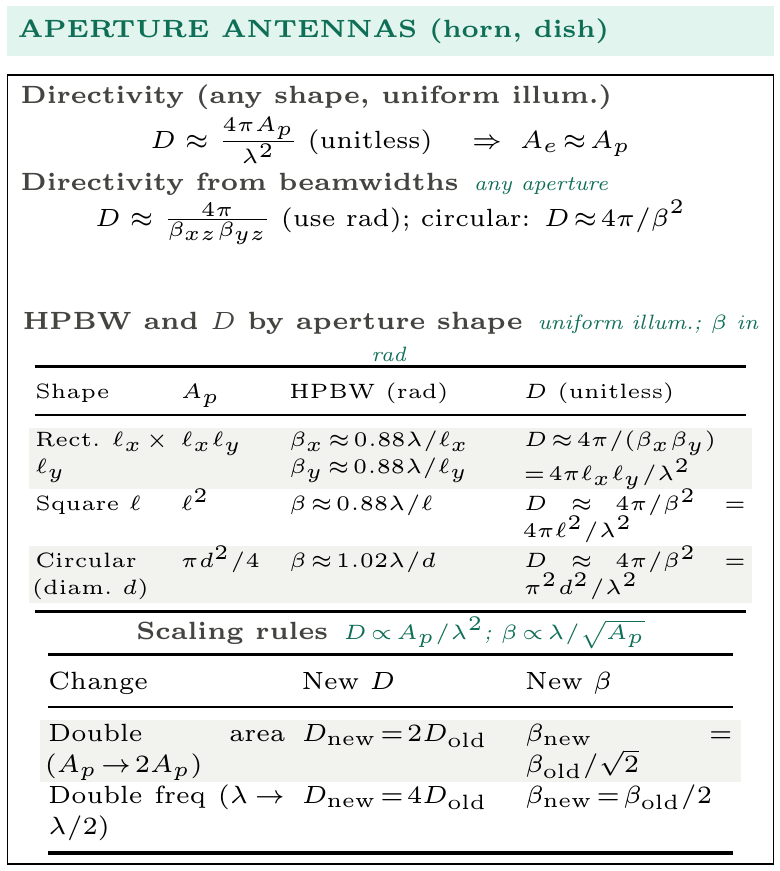
\includegraphics[width=0.49\linewidth]{cs_aperture}\hfill
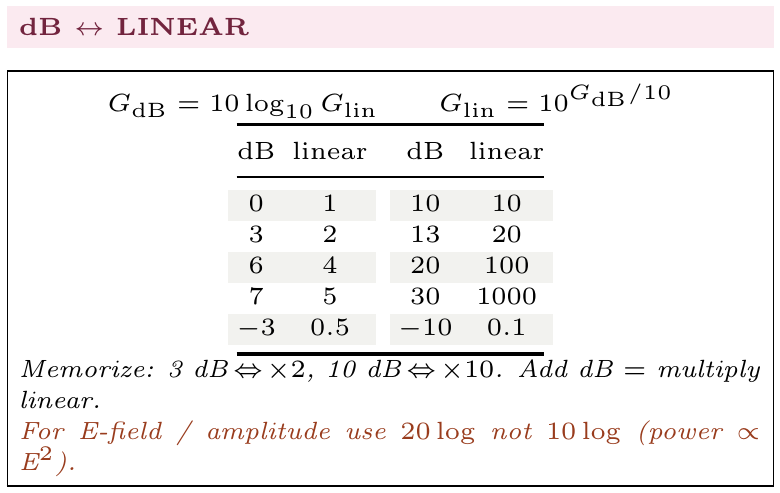
\includegraphics[width=0.49\linewidth]{cs_db}
\end{cssnip}

\vspace{6pt}
\textbf{(a) Directivity in dB (5 pts)}

\begin{goalbox}
\goal{find $D$ using the circular-beam formula (from APERTURE ANTENNAS box):}
\[D = \tfrac{4\pi}{\beta^2}\quad(\beta\text{ in radians})\]
\need{$\beta$ in radians (given as degrees).}
\end{goalbox}

\textbf{Convert $\beta$ to radians:}
\[\beta = 3^\circ \cdot \tfrac{\pi}{180} = \tfrac{\pi}{60} = 0.05236~\text{rad}\]

\textbf{Plug in:}
\[D = \tfrac{4\pi}{(0.05236)^2} = \tfrac{12.566}{0.002742} = 4584\]
\[\boxed{D = 10\log_{10}(4584) = 36.6~\text{dB}}\]

\vspace{6pt}
\textbf{(b) Area doubled $A_p \to 2A_p$ (5 pts)}

\begin{goalbox}
\goal{find new $D$ and $\beta$ using the scaling rules (from APERTURE ANTENNAS box coral note):}
\[D \propto A_p\;\Rightarrow\;D_{\text{new}} = 2D_{\text{old}}\]
\[\beta \propto 1/\sqrt{A_p}\;\Rightarrow\;\beta_{\text{new}} = \beta_{\text{old}}/\sqrt{2}\]
\need{$D_{\text{old}}$ and $\beta_{\text{old}}$ (from part a).}
\end{goalbox}

\textbf{Plug in:}
\[D_{\text{new}} = 2(4584) = 9168 \;\Rightarrow\; \boxed{D_{\text{new}} = 39.6~\text{dB}}\]
\[\beta_{\text{new}} = 3^\circ/\sqrt{2} = 3^\circ/1.414 = \boxed{2.12^\circ}\]

\vspace{6pt}
\textbf{(c) Frequency doubled $f \to 2f$ ($\lambda \to \lambda/2$), same $A_p$ (5 pts)}

\begin{goalbox}
\goal{find new $D$ and $\beta$ using scaling: from $D = 4\pi A_p/\lambda^2$ we have $D \propto 1/\lambda^2$. Halving $\lambda$ quadruples $D$. And $\beta \propto \lambda$, so halving $\lambda$ halves $\beta$.}
\need{$D_{\text{old}}$ and $\beta_{\text{old}}$ (from part a).}
\end{goalbox}

\textbf{Plug in:}
\[D_{\text{new}} = 4D_{\text{old}} = 4(4584) = 18336 \;\Rightarrow\; \boxed{D_{\text{new}} = 42.6~\text{dB}}\]
\[\beta_{\text{new}} = \beta_{\text{old}}/2 = 3^\circ/2 = \boxed{1.5^\circ}\]

\textit{Sanity:} bigger area or shorter wavelength both sharpen the beam. Doubling area: $+3$ dB ($\times 2$). Doubling frequency: $+6$ dB ($\times 4$) because both $D \propto A_p/\lambda^2$ and $1/\beta^2 \propto D$.

\newpage
%======================================================
\probhead{8 --- 5-Element Linear Array, $d = 3\lambda/4$}{(new)}

\textbf{Setup:} Broadside linear array, $N = 5$ elements, equal-phase, uniform amplitude, spacing $d = 3\lambda/4$. Find (a) normalized array factor, (b) HPBW.

\begin{cssnip}
\begin{center}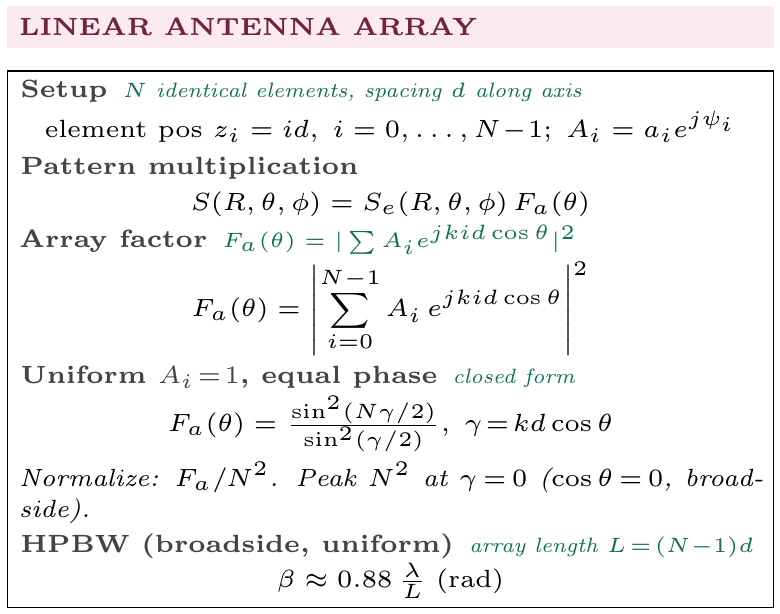
\includegraphics[width=0.55\linewidth]{cs_array}\end{center}
\end{cssnip}

\vspace{6pt}
\textbf{(a) Normalized array factor $F_a^{\text{norm}}(\theta)$ (5 pts)}

\begin{goalbox}
\goal{find $F_a^{\text{norm}}(\theta)$ using the uniform-array closed form (from LINEAR ANTENNA ARRAY box):}
\[F_a(\theta) = \tfrac{\sin^2(N\gamma/2)}{\sin^2(\gamma/2)},\quad \gamma = kd\cos\theta\]
\need{$N$, $k$, $d$, then form $\gamma$, then normalize by peak $N^2$.}
\end{goalbox}

\textbf{Solve each unknown:}

\textit{$N$:} given.
\[N = 5\]

\textit{$k$:} wavenumber.
\[k = \tfrac{2\pi}{\lambda}\]

\textit{$d$:} given.
\[d = \tfrac{3\lambda}{4}\]

\textit{$\gamma$:} combine.
\[\gamma = kd\cos\theta = \tfrac{2\pi}{\lambda}\cdot\tfrac{3\lambda}{4}\cos\theta = \tfrac{3\pi}{2}\cos\theta\]
So $N\gamma/2 = (5/2)(3\pi/2)\cos\theta = (15\pi/4)\cos\theta$ and $\gamma/2 = (3\pi/4)\cos\theta$.

\textbf{Plug into $F_a$:}
\[F_a(\theta) = \tfrac{\sin^2((15\pi/4)\cos\theta)}{\sin^2((3\pi/4)\cos\theta)}\]
Peak occurs at $\gamma = 0$ ($\cos\theta = 0$, broadside $\theta = \pi/2$): $F_a^{\text{max}} = N^2 = 25$.

\textbf{Normalize:}
\[\boxed{F_a^{\text{norm}}(\theta) = \tfrac{1}{25}\tfrac{\sin^2((15\pi/4)\cos\theta)}{\sin^2((3\pi/4)\cos\theta)}}\]

\vspace{6pt}
\textbf{(b) Half-power beamwidth $\beta$ (3 pts)}

\begin{goalbox}
\goal{find $\beta$ using the uniform-broadside-array HPBW formula:}
\[\beta \approx 0.886\tfrac{\lambda}{Nd}\quad(\text{rad})\]
\need{$N$, $d$, $\lambda$.}
\end{goalbox}

\textbf{Plug in:}
\[Nd = 5\cdot\tfrac{3\lambda}{4} = \tfrac{15\lambda}{4}\]
\[\beta = 0.886\cdot\tfrac{\lambda}{15\lambda/4} = 0.886\cdot\tfrac{4}{15} = 0.236~\text{rad}\]
\[\boxed{\beta = 0.236~\text{rad} = 13.5^\circ}\]

\textit{Cross-check by solving $F_a^{\text{norm}} = 0.5$ numerically:} get $\gamma/2 \approx 0.28$ rad, so $\cos\theta = 0.28/(3\pi/4) = 0.119$, $\theta = 83.2^\circ$, offset from broadside ($90^\circ$) by $6.8^\circ$, full HPBW $\approx 13.6^\circ$ $\checkmark$.

\textit{Sanity:} 5 elements give a moderately narrow beam ($\sim 14^\circ$) vs.\ a single dipole's $\sim 78^\circ$. Adding more elements or wider spacing narrows further (with grating-lobe risk if $d > \lambda$).

\end{document}
